
\documentclass[10pt]{beamer}
\usetheme{metropolis}

% ── Packages ──
\usepackage{amsmath,amssymb,amsthm}
\usepackage{tikz}
\usetikzlibrary{positioning,arrows.meta,fit,matrix,backgrounds,calc,shapes.geometric,3d}
\usepackage{graphicx}
\usepackage{array}
\usepackage{etoolbox}

% ── Theorem environments ──
\theoremstyle{definition}
\newtheorem{defi}{Definition}[section]
\newtheorem{prop}{Proposition}[section]
\newtheorem{thm}{Theorem}[section]
\newtheorem{cor}{Corollary}[section]

% Custom theorem styles with colors
\setbeamercolor{block title}{bg=red!75!black,fg=white}
\setbeamercolor{block body}{bg=yellow!10!white}

\AtBeginEnvironment{prop}{%
  \setbeamercolor{block title}{bg=yellow!75!black,fg=black}%
  \setbeamercolor{block body}{bg=yellow!10!white}%
}
\AtEndEnvironment{prop}{%
  \setbeamercolor{block title}{bg=red!75!black,fg=white}%
}

\AtBeginEnvironment{thm}{%
  \setbeamercolor{block title}{bg=yellow!75!black,fg=black}%
  \setbeamercolor{block body}{bg=yellow!10!white}%
}
\AtEndEnvironment{thm}{%
  \setbeamercolor{block title}{bg=red!75!black,fg=white}%
}

\AtBeginEnvironment{cor}{%
  \setbeamercolor{block title}{bg=yellow!75!black,fg=black}%
  \setbeamercolor{block body}{bg=yellow!10!white}%
}
\AtEndEnvironment{cor}{%
  \setbeamercolor{block title}{bg=red!75!black,fg=white}%
}

% ── Highlighting ──
\newcommand{\x}[1]{\alert{\textbf{#1}}}

% ── Cross-filling colors ──
\newcommand{\pvt}[1]{{\color{red}\mathbf{#1}}}       % pivot
\newcommand{\crs}[1]{{\color{blue}#1}}                % cross arm
\newcommand{\gn}[1]{{\color{green!60!black}#1}}       % green highlight
\newcommand{\rd}[1]{{\color{red}#1}}                  % red highlight
\newcommand{\bl}[1]{{\color{blue}#1}}                 % blue highlight
\newcommand{\tl}[1]{{\color{teal}#1}}                 % teal highlight
\newcommand{\gz}{{\color{gray}0}}                      % gray zero (consumed)

\title{Lecture 11: Linear Regression}
\subtitle{MATH203 Applied Linear Algebra}
\date{}
\titlegraphic{}

\begin{document}
\maketitle


% ═══════════════════════════════════════
% §1 THE CANDLE PROBLEM
% ADR: AUDIENCE EMOTION — students need a REAL problem before any math.
% A burning candle is visceral: everyone has seen it. The question
% "when does it burn out?" is immediately meaningful.
% No matrices, no equations, no R^n — just a candle and a ruler.
% Structure: observe → question → candidate answers → what is "best"?
% ═══════════════════════════════════════
\section{The Candle Problem}


% ADR: AUDIENCE EMOTION — pure visual. No math. Just a candle getting shorter.
% The 3 candles at different times ARE the data. Students see the pattern
% before being told there is one.
\begin{frame}[fragile]{A Burning Candle}

You light a candle and measure its height over time.

\vspace{1em}

\begin{center}
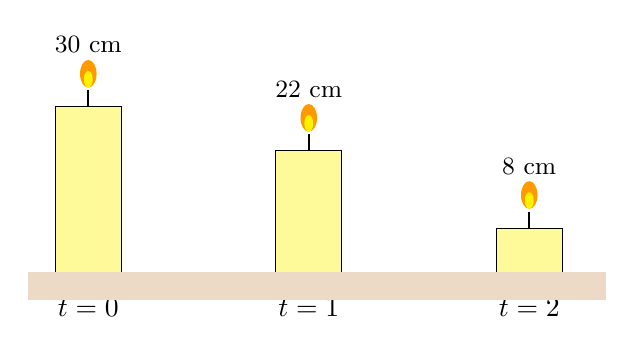
\begin{tikzpicture}[scale=0.7]
  % Candle 1: t=0, h=30cm
  \fill[yellow!40] (0,0) rectangle (1.2,3.0);
  \draw (0,0) rectangle (1.2,3.0);
  % wick
  \draw[thick] (0.6,3.0) -- (0.6,3.3);
  % flame
  \fill[orange!80!yellow] (0.6,3.6) ellipse (0.15 and 0.25);
  \fill[yellow] (0.6,3.5) ellipse (0.08 and 0.15);
  \node[below] at (0.6,-0.3) {$t = 0$};
  \node[above] at (0.6,3.8) {\small 30 cm};

  % Candle 2: t=1, h=22cm
  \fill[yellow!40] (4,0) rectangle (5.2,2.2);
  \draw (4,0) rectangle (5.2,2.2);
  \draw[thick] (4.6,2.2) -- (4.6,2.5);
  \fill[orange!80!yellow] (4.6,2.8) ellipse (0.15 and 0.25);
  \fill[yellow] (4.6,2.7) ellipse (0.08 and 0.15);
  \node[below] at (4.6,-0.3) {$t = 1$};
  \node[above] at (4.6,3.0) {\small 22 cm};

  % Candle 3: t=2, h=8cm
  \fill[yellow!40] (8,0) rectangle (9.2,0.8);
  \draw (8,0) rectangle (9.2,0.8);
  \draw[thick] (8.6,0.8) -- (8.6,1.1);
  \fill[orange!80!yellow] (8.6,1.4) ellipse (0.15 and 0.25);
  \fill[yellow] (8.6,1.3) ellipse (0.08 and 0.15);
  \node[below] at (8.6,-0.3) {$t = 2$};
  \node[above] at (8.6,1.6) {\small 8 cm};

  % table surface
  \fill[brown!30] (-0.5,-0.5) rectangle (10,0);
\end{tikzpicture}
\end{center}

\end{frame}


% ADR: AUDIENCE EMOTION — formalize the observation as a data table + scatter plot.
% Still no model, no formula. Just "here is what we measured."
\begin{frame}[fragile]{The Data}

\begin{columns}
\column{0.4\textwidth}
\begin{center}
\begin{tabular}{|c|c|}
\hline
Time (hours) & Height (cm) \\
\hline
0 & 30 \\
1 & 22 \\
2 & 8 \\
\hline
\end{tabular}
\end{center}

\column{0.6\textwidth}
\begin{center}
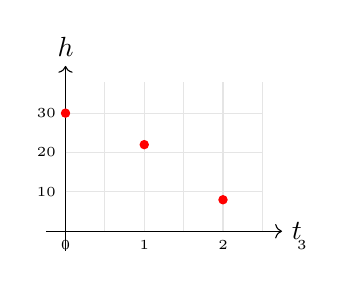
\begin{tikzpicture}[scale=0.5]
  % axes
  \draw[->] (-0.5,0) -- (5.5,0) node[right] {$t$};
  \draw[->] (0,-0.5) -- (0,4.2) node[above] {$h$};
  % grid
  \foreach \x in {1,...,5} \draw[gray!20] (\x,0) -- (\x,3.8);
  \foreach \y in {1,...,3} \draw[gray!20] (0,\y) -- (5,\y);
  % tick labels (t-scale: 1 unit = 2 on x-axis)
  \foreach \x in {0,1,2,3} \node[below,font=\tiny] at (2*\x,0) {\x};
  \node[left,font=\tiny] at (0,1) {10};
  \node[left,font=\tiny] at (0,2) {20};
  \node[left,font=\tiny] at (0,3) {30};
  % data points (t=0,1,2 → x=0,2,4; h/10 → y)
  \fill[red] (0,3) circle (0.12);
  \fill[red] (2,2.2) circle (0.12);
  \fill[red] (4,0.8) circle (0.12);
\end{tikzpicture}
\end{center}
\end{columns}

\vspace{1em}

The candle gets shorter over time. \x{Can we predict its height at $t = 3$?}

\end{frame}


% ADR: AUDIENCE EMOTION — intuition: "draw a line through the points."
% Show multiple candidate lines so students see there's a CHOICE to make.
\begin{frame}[fragile]{Drawing a Line}

Our instinct: draw a straight line through the data.

\vspace{0.5em}

\begin{center}
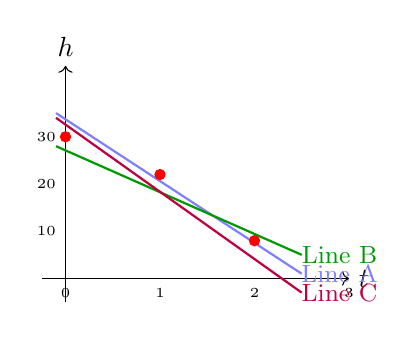
\begin{tikzpicture}[scale=0.6]
  % axes (t-scale: 1 unit = 2 on x-axis)
  \draw[->] (-0.5,0) -- (6,0) node[right] {$t$};
  \draw[->] (0,-0.5) -- (0,4.5) node[above] {$h$};
  \foreach \x in {0,1,2,3} \node[below,font=\tiny] at (2*\x,0) {\x};
  \node[left,font=\tiny] at (0,1) {10};
  \node[left,font=\tiny] at (0,2) {20};
  \node[left,font=\tiny] at (0,3) {30};
  % candidate lines (t=0..2, x=0..4)
  \draw[blue!50,thick] (-0.2,3.5) -- (5,0.1);
  \node[blue!50,font=\small] at (5.8,0.1) {Line A};
  \draw[green!60!black,thick] (-0.2,2.8) -- (5,0.5);
  \node[green!60!black,font=\small] at (5.8,0.5) {Line B};
  \draw[purple,thick] (-0.2,3.4) -- (5,-0.3);
  \node[purple,font=\small] at (5.8,-0.3) {Line C};
  % data points (on top)
  \fill[red] (0,3) circle (0.12);
  \fill[red] (2,2.2) circle (0.12);
  \fill[red] (4,0.8) circle (0.12);
\end{tikzpicture}
\end{center}

\vspace{0.5em}

Three different lines. Which one is the \x{best}?

\end{frame}


% ADR: AUDIENCE EMOTION — define "best" visually: vertical gaps on the plot.
% Pick a not-great line so gaps are visible. Label each gap with a NUMBER.
% No algebra. No "a - 30". Just picture + numbers.
\begin{frame}[fragile]{What Does ``Best'' Mean?}

Pick a line (not a great fit). Measure the \x{vertical gap} at each data point.

\vspace{0.3em}

\begin{center}
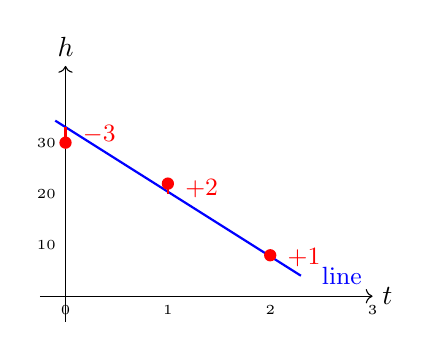
\begin{tikzpicture}[scale=0.65]
  % axes (t-scale: 1 unit = 2 on x-axis)
  \draw[->] (-0.5,0) -- (6,0) node[right] {$t$};
  \draw[->] (0,-0.5) -- (0,4.5) node[above] {$h$};
  \foreach \x in {0,1,2,3} \node[below,font=\tiny] at (2*\x,0) {\x};
  \node[left,font=\tiny] at (0,1) {10};
  \node[left,font=\tiny] at (0,2) {20};
  \node[left,font=\tiny] at (0,3) {30};
  % a not-great line: h = 33 - 13t (plot: y = 3.3 - 1.3t, x = 2t)
  % t=0: y=3.3, t=2: y=0.7 → x=0: 3.3, x=4: 0.7
  \draw[blue,thick] (-0.2,3.43) -- (4.6,0.4);
  \node[blue,font=\small] at (5.4,0.4) {line};
  % line values at data points:
  % t=0: line=3.3 (33cm), data=3.0 (30cm), gap = -3
  % t=1: line=2.0 (20cm), data=2.2 (22cm), gap = +2
  % t=2: line=0.7 (7cm),  data=0.8 (8cm),  gap = +1
  % gap lines
  \draw[red,thick] (0,3.3) -- (0,3.0);
  \node[red,font=\small,right] at (0.15,3.15) {$-3$};
  \draw[red,thick] (2,2.0) -- (2,2.2);
  \node[red,font=\small,right] at (2.15,2.1) {$+2$};
  \draw[red,thick] (4,0.7) -- (4,0.8);
  \node[red,font=\small,right] at (4.15,0.75) {$+1$};
  % data points (on top)
  \fill[red] (0,3) circle (0.12);
  \fill[red] (2,2.2) circle (0.12);
  \fill[red] (4,0.8) circle (0.12);
\end{tikzpicture}
\end{center}

\vspace{0.3em}

Three gaps: $-3$, $+2$, $+1$.

\end{frame}


% ADR: AUDIENCE EMOTION — the error is just "sum of squares of those three numbers."
% Show it as arithmetic, not algebra. Then state the goal.
\begin{frame}{The Error}

How bad is this line? Add up the squared gaps:

$$\text{Error} = (-3)^2 + (+2)^2 + (+1)^2 = 9 + 4 + 1 = 14$$

\vspace{1em}

A different line would give different gaps, and a different error.

\vspace{1em}

\x{Goal}: Find the line whose error is the \x{smallest possible}.

\end{frame}


% ADR: AUDIENCE EMOTION — tension. No calculus, no "approach."
% Just: this is hard to do by trial and error. Geometry will help.
\begin{frame}{How?}

We could try thousands of lines and pick the one with the smallest error.

\vspace{1em}

But there is a \x{geometric shortcut}.

\vspace{1em}

We will translate this problem into a picture in $\mathbb{R}^3$, where the answer becomes \x{obvious}.

\end{frame}


% ═══════════════════════════════════════
% §2 DATA AS GEOMETRY
% ADR: AUDIENCE EMOTION — this is the MAIN insight of the lecture.
% The translation from "data fitting" to "projection" deserves many frames.
% Three sub-steps, each with its own visual:
%   A. Data = a point in R³
%   B. Model family = a plane (subspace) in R³
%   C. Error = distance (later section)
%
% The chopstick-marble metaphor is the concretization for Step A.
% For Step B, we compute specific "perfect data" vectors to show
% that they all live on a plane.
% ═══════════════════════════════════════
\section{Data as Geometry}


% ─────────────────────────────
% Step A: Data = a point in R³
% ─────────────────────────────

% ADR: AUDIENCE EMOTION — start with the raw observation:
% "you have 3 numbers." Nothing more.
\begin{frame}{Three Measurements}

Your experiment produced \x{three numbers}:

\vspace{1em}

\begin{center}
\begin{tabular}{ccc}
\large $h_1 = 30$ & \large $h_2 = 22$ & \large $h_3 = 8$
\end{tabular}
\end{center}

\vspace{1em}

That is all the information you have about this candle.

\vspace{0.5em}

Three numbers. Can we think of them as \x{one object}?

\end{frame}


% ADR: AUDIENCE EMOTION — the chopstick-marble visual.
% Each chopstick is a number line. Each marble marks one measurement.
% Three chopsticks = three axes. This is R³ before we say "R³".
\begin{frame}[fragile]{Marbles on Chopsticks}

Imagine three \x{chopsticks} standing upright. Place a marble on each one at the measured height.

\vspace{0.5em}

\begin{center}
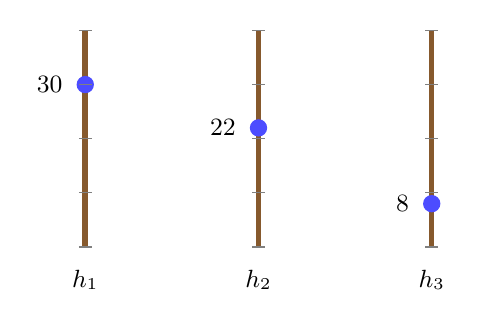
\begin{tikzpicture}[scale=0.55]
  % Chopstick 1
  \draw[brown!70!black, line width=2pt] (0,0) -- (0,5);
  \fill[blue!70] (0,3.75) circle (0.2);
  \node[left,font=\small] at (-0.3,3.75) {$30$};
  \node[below,font=\small] at (0,-0.3) {$h_1$};
  % scale ticks
  \foreach \y/\lab in {0/0, 1.25/10, 2.5/20, 3.75/30, 5/40}
    \draw[gray] (-0.15,\y) -- (0.15,\y);

  % Chopstick 2
  \draw[brown!70!black, line width=2pt] (4,0) -- (4,5);
  \fill[blue!70] (4,2.75) circle (0.2);
  \node[left,font=\small] at (3.7,2.75) {$22$};
  \node[below,font=\small] at (4,-0.3) {$h_2$};
  \foreach \y/\lab in {0/0, 1.25/10, 2.5/20, 3.75/30, 5/40}
    \draw[gray] (3.85,\y) -- (4.15,\y);

  % Chopstick 3
  \draw[brown!70!black, line width=2pt] (8,0) -- (8,5);
  \fill[blue!70] (8,1.0) circle (0.2);
  \node[left,font=\small] at (7.7,1.0) {$8$};
  \node[below,font=\small] at (8,-0.3) {$h_3$};
  \foreach \y/\lab in {0/0, 1.25/10, 2.5/20, 3.75/30, 5/40}
    \draw[gray] (7.85,\y) -- (8.15,\y);
\end{tikzpicture}
\end{center}

\vspace{0.3em}

Three chopsticks. Three marbles. The \x{positions of all three marbles together} describe your experiment.

\end{frame}


% ADR: AUDIENCE EMOTION — the AHA: three chopsticks = three coordinate axes.
% The marble configuration = one point in 3D space.
\begin{frame}[fragile]{Three Chopsticks = Three Axes}

Now tilt the chopsticks into three perpendicular directions.

\begin{center}
\begin{tikzpicture}[scale=0.6]
  % 3D axes
  \draw[->,thick] (0,0) -- (4.5,0) node[right] {$h_1$};
  \draw[->,thick] (0,0) -- (-2,-2) node[below left] {$h_2$};
  \draw[->,thick] (0,0) -- (0,4) node[above] {$h_3$};

  % The point (30, 22, 8) in projected coords
  \coordinate (P) at (1.6, 0.8);

  % projection guides (dashed)
  \draw[dashed, gray] (3.0,0) -- (1.6,0) -- (1.6,0.8);
  \draw[dashed, gray] (0,0.8) -- (1.6,0.8);
  \draw[dashed, gray] (-1.4,-1.4) -- (1.6,-1.4) -- (1.6,0);

  % the point
  \fill[red] (P) circle (0.12);
  \node[red, right, font=\small] at (1.8,0.9) {$(30,\; 22,\; 8)$};

  % axis labels
  \node[below,font=\tiny] at (3.0,0) {$30$};
  \node[below left,font=\tiny] at (-1.4,-1.4) {$22$};
  \node[left,font=\tiny] at (0,0.8) {$8$};
\end{tikzpicture}
\end{center}

The three marble positions become \x{one point} in 3-dimensional space:
$\mathbf{b} = (30,\; 22,\; 8)^T \in \mathbb{R}^3$

\end{frame}


% ADR: AUDIENCE EMOTION — reinforce: different data → different point.
% The concept "data = point" must feel inevitable, not arbitrary.
\begin{frame}[fragile]{Different Candle, Different Point}

If you repeated the experiment with a different candle:

\vspace{0.3em}

\begin{center}
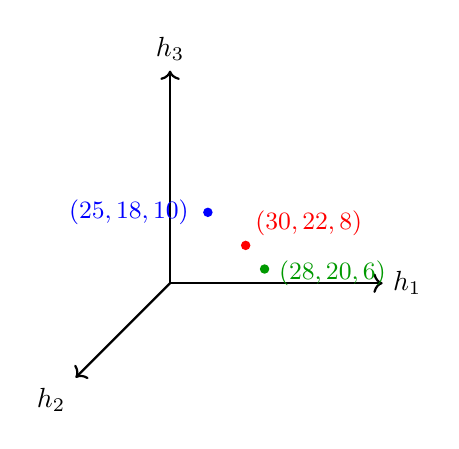
\begin{tikzpicture}[scale=0.6]
  % 3D axes
  \draw[->,thick] (0,0) -- (4.5,0) node[right] {$h_1$};
  \draw[->,thick] (0,0) -- (-2,-2) node[below left] {$h_2$};
  \draw[->,thick] (0,0) -- (0,4.5) node[above] {$h_3$};

  % Original point
  \fill[red] (1.6,0.8) circle (0.1);
  \node[red, font=\small, above right] at (1.6,0.8) {$(30, 22, 8)$};

  % Another experiment: say (25, 18, 10)
  \fill[blue] (0.8,1.5) circle (0.1);
  \node[blue, font=\small, left] at (0.6,1.5) {$(25, 18, 10)$};

  % Yet another: (28, 20, 6)
  \fill[green!60!black] (2.0,0.3) circle (0.1);
  \node[green!60!black, font=\small, right] at (2.1,0.2) {$(28, 20, 6)$};
\end{tikzpicture}
\end{center}

\vspace{0.3em}

Every possible experiment produces some point in $\mathbb{R}^3$.

\vspace{0.5em}

\x{All of the candle's data lives in one place}: the space $\mathbb{R}^3$.

\end{frame}


% ADR: AUDIENCE EMOTION — summary of Step A. Pause before moving on.
\begin{frame}{Data = A Point}

\begin{center}
\large
3 measurements on a number line

$\Big\Downarrow$

\vspace{0.5em}

1 point in $\mathbb{R}^3$
\end{center}

\vspace{1em}

Our candle experiment gave us:

$$\mathbf{b} = \begin{pmatrix} 30 \\ 22 \\ 8 \end{pmatrix}$$

\vspace{0.5em}

This is our \x{observed data}, living as a single point in $\mathbb{R}^3$.

\end{frame}


% ─────────────────────────────
% Step B: Model = a plane in R³
% ADR: KEY INSIGHT — there are TWO spaces:
%   1. The scatter plot (2D, where we see data points and lines)
%   2. The data space (R³, where each experiment is ONE point)
% Perfect data in the scatter plot (3 points on a line) becomes
% a single point on a PLANE in data space.
% CRITICAL: the plane depends on the CHOPSTICK POSITIONS (time points).
% Different measurement times → different plane. Must show this with
% multiple diagrams.
% ─────────────────────────────

% ADR: AUDIENCE EMOTION — pause and distinguish the two spaces.
% Students have just learned "3 measurements = 1 point in R³."
% Now prevent confusion: the scatter plot is NOT the same as data space.
\begin{frame}[fragile]{Two Different Pictures}

\begin{columns}
\column{0.48\textwidth}
\begin{center}
\textbf{Scatter plot}

\vspace{0.3em}

\begin{tikzpicture}[scale=0.4]
  \draw[->] (-0.5,0) -- (5.5,0) node[right] {\tiny $t$};
  \draw[->] (0,-0.5) -- (0,4.2) node[above] {\tiny $h$};
  \fill[red] (0,3) circle (0.12);
  \fill[red] (2,2.2) circle (0.12);
  \fill[red] (4,0.8) circle (0.12);
\end{tikzpicture}

\vspace{0.3em}

3 dots in 2D

\small Each dot = one measurement
\end{center}

\column{0.48\textwidth}
\begin{center}
\textbf{Data space}

\vspace{0.3em}

\begin{tikzpicture}[scale=0.4]
  \draw[->,thick] (0,0) -- (3.5,0) node[right] {\tiny $h_1$};
  \draw[->,thick] (0,0) -- (-1.5,-1.5) node[below left] {\tiny $h_2$};
  \draw[->,thick] (0,0) -- (0,3.5) node[above] {\tiny $h_3$};
  \fill[red] (1.2,0.5) circle (0.12);
\end{tikzpicture}

\vspace{0.3em}

1 dot in 3D

\small The dot = all three measurements together
\end{center}
\end{columns}

\vspace{0.5em}

These are \x{two completely different spaces}. Do not confuse them.

\end{frame}


% ADR: AUDIENCE EMOTION — what is "perfect data"? Show it on CHOPSTICKS:
% marbles on 3 chopsticks, connected by a line → they're collinear!
% Perfect = the marbles line up. Imperfect = they don't.
\begin{frame}[fragile]{What Is ``Perfect Data''?}

Place marbles on the chopsticks. If the marble tops form a \x{straight line}: perfect!

\vspace{0.3em}

\begin{center}
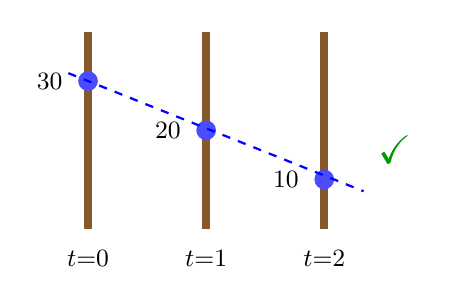
\begin{tikzpicture}[scale=0.5]
  % chopsticks at t=0, 1, 2 (visual: x=0, 3, 6)
  \draw[brown!70!black, line width=3pt] (0,0) -- (0,5);
  \draw[brown!70!black, line width=3pt] (3,0) -- (3,5);
  \draw[brown!70!black, line width=3pt] (6,0) -- (6,5);
  \node[below,font=\small] at (0,-0.3) {$t{=}0$};
  \node[below,font=\small] at (3,-0.3) {$t{=}1$};
  \node[below,font=\small] at (6,-0.3) {$t{=}2$};
  % perfect marbles: heights 30, 20, 10 (scale: /8)
  \fill[blue!70] (0,3.75) circle (0.25);
  \fill[blue!70] (3,2.5) circle (0.25);
  \fill[blue!70] (6,1.25) circle (0.25);
  \node[left,font=\small] at (-0.4,3.75) {$30$};
  \node[left,font=\small] at (2.6,2.5) {$20$};
  \node[left,font=\small] at (5.6,1.25) {$10$};
  % line through marbles
  \draw[blue,thick,dashed] (-0.5,3.95) -- (7,0.95);
  % checkmark
  \node[green!60!black,font=\Large] at (7.8,2) {$\checkmark$};
\end{tikzpicture}
\end{center}

\vspace{0.3em}

The marbles at $30$, $20$, $10$ lie on a straight line. \x{Perfect data.}

\end{frame}


% ADR: AUDIENCE EMOTION — contrast: our actual data is NOT perfect.
% Same chopsticks, but marbles don't line up.
\begin{frame}[fragile]{Our Data Is Not Perfect}

Now put our \x{actual} marbles on the same chopsticks:

\vspace{0.3em}

\begin{center}
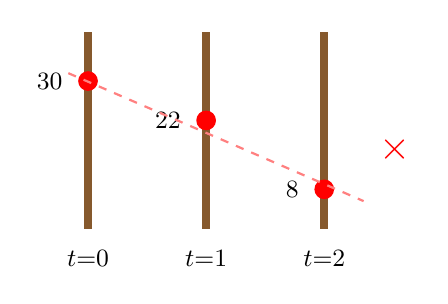
\begin{tikzpicture}[scale=0.5]
  % chopsticks at t=0, 1, 2 (visual: x=0, 3, 6)
  \draw[brown!70!black, line width=3pt] (0,0) -- (0,5);
  \draw[brown!70!black, line width=3pt] (3,0) -- (3,5);
  \draw[brown!70!black, line width=3pt] (6,0) -- (6,5);
  \node[below,font=\small] at (0,-0.3) {$t{=}0$};
  \node[below,font=\small] at (3,-0.3) {$t{=}1$};
  \node[below,font=\small] at (6,-0.3) {$t{=}2$};
  % actual marbles: 30, 22, 8 (scale: /8)
  \fill[red] (0,3.75) circle (0.25);
  \fill[red] (3,2.75) circle (0.25);
  \fill[red] (6,1.0) circle (0.25);
  \node[left,font=\small] at (-0.4,3.75) {$30$};
  \node[left,font=\small] at (2.6,2.75) {$22$};
  \node[left,font=\small] at (5.6,1.0) {$8$};
  % try to draw a line — doesn't go through all
  \draw[red!50,thick,dashed] (-0.5,3.95) -- (7,0.7);
  % cross
  \node[red,font=\Large] at (7.8,2) {$\times$};
\end{tikzpicture}
\end{center}

\vspace{0.3em}

$30$, $22$, $8$ do \x{not} lie on any straight line. Our data is imperfect.

\end{frame}


% ADR: AUDIENCE EMOTION — NOW the critical insight: the chopstick positions
% DEFINE what "lining up" means. Move the chopsticks → same marbles might
% or might not line up. Must show this visually with marbles + line.
\begin{frame}[fragile]{Chopstick Positions Define ``Perfect''}

The \x{same marble heights} can be perfect or imperfect --- depending on \x{where the chopsticks are}!

\vspace{0.3em}

\begin{columns}
\column{0.48\textwidth}
\begin{center}
\small Chopsticks at $t = 0, 1, 2$

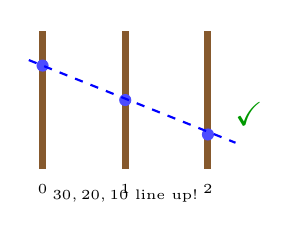
\begin{tikzpicture}[scale=0.35]
  % chopsticks (visual: x=0, 3, 6)
  \draw[brown!70!black, line width=2.5pt] (0,0) -- (0,5);
  \draw[brown!70!black, line width=2.5pt] (3,0) -- (3,5);
  \draw[brown!70!black, line width=2.5pt] (6,0) -- (6,5);
  \node[below,font=\tiny] at (0,-0.2) {$0$};
  \node[below,font=\tiny] at (3,-0.2) {$1$};
  \node[below,font=\tiny] at (6,-0.2) {$2$};
  % marbles at 30, 20, 10 (scale /8)
  \fill[blue!70] (0,3.75) circle (0.22);
  \fill[blue!70] (3,2.5) circle (0.22);
  \fill[blue!70] (6,1.25) circle (0.22);
  % line
  \draw[blue,thick,dashed] (-0.5,3.95) -- (7,0.95);
  \node[green!60!black,font=\large] at (7.5,2) {$\checkmark$};
  \node[font=\tiny] at (3,-1) {$30, 20, 10$ line up!};
\end{tikzpicture}
\end{center}

\column{0.48\textwidth}
\begin{center}
\small Chopsticks at $t = 0, 1, 3$

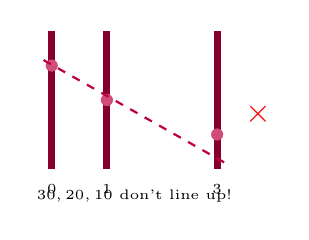
\begin{tikzpicture}[scale=0.35]
  % chopsticks at different positions (visual: x=0, 2, 6)
  \draw[purple!70!black, line width=2.5pt] (0,0) -- (0,5);
  \draw[purple!70!black, line width=2.5pt] (2,0) -- (2,5);
  \draw[purple!70!black, line width=2.5pt] (6,0) -- (6,5);
  \node[below,font=\tiny] at (0,-0.2) {$0$};
  \node[below,font=\tiny] at (2,-0.2) {$1$};
  \node[below,font=\tiny] at (6,-0.2) {$3$};
  % SAME marble heights: 30, 20, 10
  \fill[purple!70] (0,3.75) circle (0.22);
  \fill[purple!70] (2,2.5) circle (0.22);
  \fill[purple!70] (6,1.25) circle (0.22);
  % line through first and second → at t=3 gives 0, not 10
  \draw[purple,thick,dashed] (-0.3,3.95) -- (6.5,0.1);
  \node[red,font=\large] at (7.5,2) {$\times$};
  \node[font=\tiny] at (3,-1) {$30, 20, 10$ don't line up!};
\end{tikzpicture}
\end{center}
\end{columns}

\vspace{0.5em}

\x{You need the chopstick positions first, then you can say what is ``perfect.''}

\end{frame}


% ADR: AUDIENCE EMOTION — different chopstick positions → different
% perfect marble heights for the SAME line. Show two chopstick configs
% each with their own perfect marbles.
\begin{frame}[fragile]{Different Chopsticks, Different Perfect Data}

For the same burning rate, the \x{perfect marble heights} change when you move the chopsticks.

\vspace{0.3em}

\begin{columns}
\column{0.48\textwidth}
\begin{center}
\small Chopsticks at $t = 0, 1, 2$

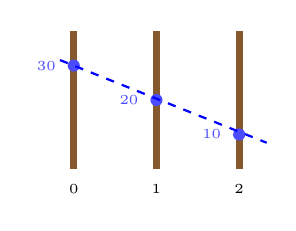
\begin{tikzpicture}[scale=0.35]
  \draw[brown!70!black, line width=2.5pt] (0,0) -- (0,5);
  \draw[brown!70!black, line width=2.5pt] (3,0) -- (3,5);
  \draw[brown!70!black, line width=2.5pt] (6,0) -- (6,5);
  \node[below,font=\tiny] at (0,-0.2) {$0$};
  \node[below,font=\tiny] at (3,-0.2) {$1$};
  \node[below,font=\tiny] at (6,-0.2) {$2$};
  % perfect: 30, 20, 10 (from h=30-10t)
  \fill[blue!70] (0,3.75) circle (0.22);
  \fill[blue!70] (3,2.5) circle (0.22);
  \fill[blue!70] (6,1.25) circle (0.22);
  \draw[blue,thick,dashed] (-0.5,3.95) -- (7,0.95);
  \node[left,font=\tiny,blue!70] at (-0.3,3.75) {30};
  \node[left,font=\tiny,blue!70] at (2.7,2.5) {20};
  \node[left,font=\tiny,blue!70] at (5.7,1.25) {10};
\end{tikzpicture}

\small Perfect: $30, 20, 10$
\end{center}

\column{0.48\textwidth}
\begin{center}
\small Chopsticks at $t = 0, 1, 3$

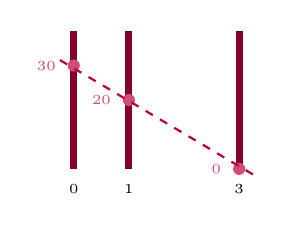
\begin{tikzpicture}[scale=0.35]
  \draw[purple!70!black, line width=2.5pt] (0,0) -- (0,5);
  \draw[purple!70!black, line width=2.5pt] (2,0) -- (2,5);
  \draw[purple!70!black, line width=2.5pt] (6,0) -- (6,5);
  \node[below,font=\tiny] at (0,-0.2) {$0$};
  \node[below,font=\tiny] at (2,-0.2) {$1$};
  \node[below,font=\tiny] at (6,-0.2) {$3$};
  % perfect for same line h=30-10t at t=0,1,3: 30, 20, 0
  \fill[purple!70] (0,3.75) circle (0.22);
  \fill[purple!70] (2,2.5) circle (0.22);
  \fill[purple!70] (6,0) circle (0.22);
  \draw[purple,thick,dashed] (-0.5,3.95) -- (6.5,-0.2);
  \node[left,font=\tiny,purple!70] at (-0.3,3.75) {30};
  \node[left,font=\tiny,purple!70] at (1.7,2.5) {20};
  \node[left,font=\tiny,purple!70] at (5.7,0) {0};
\end{tikzpicture}

\small Perfect: $30, 20, 0$
\end{center}
\end{columns}

\vspace{0.5em}

Same candle, same burning rate. But the chopstick positions changed, so the perfect marble heights are \x{completely different}.

\end{frame}


% ADR: AUDIENCE EMOTION — now show many perfect marble configurations
% for OUR chopsticks. Each config = one point in R³.
% Different lines → different perfect marbles → different points.
\begin{frame}[fragile]{Many Perfect Configurations}

Back to our chopsticks at $t = 0, 1, 2$. Here are several perfect marble sets:

\vspace{0.3em}

\begin{center}
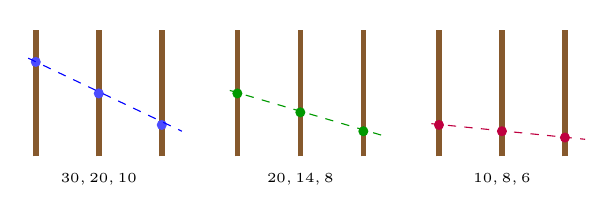
\begin{tikzpicture}[scale=0.32]
  % Config 1: 30, 20, 10 (h=30-10t)
  \draw[brown!70!black, line width=2pt] (0,0) -- (0,5);
  \draw[brown!70!black, line width=2pt] (2.5,0) -- (2.5,5);
  \draw[brown!70!black, line width=2pt] (5,0) -- (5,5);
  \fill[blue!70] (0,3.75) circle (0.2);
  \fill[blue!70] (2.5,2.5) circle (0.2);
  \fill[blue!70] (5,1.25) circle (0.2);
  \draw[blue,dashed] (-0.3,3.9) -- (5.8,1.0);
  \node[below,font=\tiny] at (2.5,-0.3) {$30, 20, 10$};

  % Config 2: 20, 14, 8 (h=20-6t)
  \begin{scope}[xshift=8cm]
  \draw[brown!70!black, line width=2pt] (0,0) -- (0,5);
  \draw[brown!70!black, line width=2pt] (2.5,0) -- (2.5,5);
  \draw[brown!70!black, line width=2pt] (5,0) -- (5,5);
  \fill[green!60!black] (0,2.5) circle (0.2);
  \fill[green!60!black] (2.5,1.75) circle (0.2);
  \fill[green!60!black] (5,1.0) circle (0.2);
  \draw[green!60!black,dashed] (-0.3,2.62) -- (5.8,0.82);
  \node[below,font=\tiny] at (2.5,-0.3) {$20, 14, 8$};
  \end{scope}

  % Config 3: 10, 8, 6 (h=10-2t)
  \begin{scope}[xshift=16cm]
  \draw[brown!70!black, line width=2pt] (0,0) -- (0,5);
  \draw[brown!70!black, line width=2pt] (2.5,0) -- (2.5,5);
  \draw[brown!70!black, line width=2pt] (5,0) -- (5,5);
  \fill[purple] (0,1.25) circle (0.2);
  \fill[purple] (2.5,1.0) circle (0.2);
  \fill[purple] (5,0.75) circle (0.2);
  \draw[purple,dashed] (-0.3,1.3) -- (5.8,0.68);
  \node[below,font=\tiny] at (2.5,-0.3) {$10, 8, 6$};
  \end{scope}
\end{tikzpicture}
\end{center}

\vspace{0.3em}

Each set of perfect marbles = one point in $\mathbb{R}^3$.

\vspace{0.3em}

\x{What shape do all these points form?}

\end{frame}


% ─────────────────────────────
% WHY IS IT A PLANE? Geometric construction with 3 special points.
% ADR: DESIGN DECISION — students cannot follow "linear combination of
% two vectors = plane." They CAN follow "here are 3 special points,
% 3 points determine a plane." So we BUILD the plane from 3 concrete
% perfect-data points that students can SEE on chopsticks:
%   Point 0: (0,0,0) = zero candle = trivially perfect
%   Point 1: (1,1,1) = all marbles at height 1 = horizontal line = perfect
%   Point 2: (0,1,2) = marbles at chopstick x-positions = diagonal line = perfect
% Each point gets its own chopstick diagram + data-space dot.
% Then: "3 points determine a plane" → done. No algebra needed.
% ─────────────────────────────

% ADR: AUDIENCE EMOTION — first special perfect data: all marbles at same height.
% This is the simplest possible perfect data: a horizontal line.
% Show it on chopsticks. No matter where the chopsticks are, level marbles
% always form a straight line. This is geometrically obvious.
\begin{frame}[fragile]{Special Perfect Data \#1: Level Marbles}

Put all marbles at the \x{same height} (say, height $1$).

\vspace{0.3em}

\begin{center}
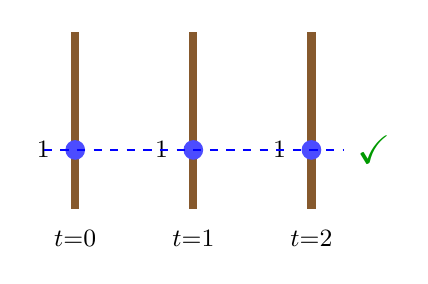
\begin{tikzpicture}[scale=0.5]
  % chopsticks at t=0, 1, 2 (visual: x=0, 3, 6)
  \draw[brown!70!black, line width=3pt] (0,0) -- (0,4.5);
  \draw[brown!70!black, line width=3pt] (3,0) -- (3,4.5);
  \draw[brown!70!black, line width=3pt] (6,0) -- (6,4.5);
  \node[below,font=\small] at (0,-0.3) {$t{=}0$};
  \node[below,font=\small] at (3,-0.3) {$t{=}1$};
  \node[below,font=\small] at (6,-0.3) {$t{=}2$};
  % marbles all at height 1 (scale: *1.5 for visibility)
  \fill[blue!70] (0,1.5) circle (0.25);
  \fill[blue!70] (3,1.5) circle (0.25);
  \fill[blue!70] (6,1.5) circle (0.25);
  \node[left,font=\small] at (-0.4,1.5) {$1$};
  \node[left,font=\small] at (2.6,1.5) {$1$};
  \node[left,font=\small] at (5.6,1.5) {$1$};
  % horizontal line through marbles
  \draw[blue,thick,dashed] (-0.8,1.5) -- (6.8,1.5);
  \node[green!60!black,font=\Large] at (7.6,1.5) {$\checkmark$};
\end{tikzpicture}
\end{center}

\vspace{0.3em}

Level marbles \x{always} form a straight line, no matter where the chopsticks are!

\vspace{0.3em}

In data space: the point $\bl{(1, 1, 1)}$.

\end{frame}


% ADR: AUDIENCE EMOTION — second special perfect data: marbles at the
% chopstick x-positions themselves. Marble on chopstick at t=0 sits at
% height 0, at t=2 sits at height 2, at t=5 sits at height 5.
% This forms a diagonal line with slope 1: h(t) = t.
% Show it clearly on chopsticks.
\begin{frame}[fragile]{Special Perfect Data \#2: Diagonal Marbles}

Put each marble at the \x{chopstick's own position}: height $= t$.

\vspace{0.3em}

\begin{center}
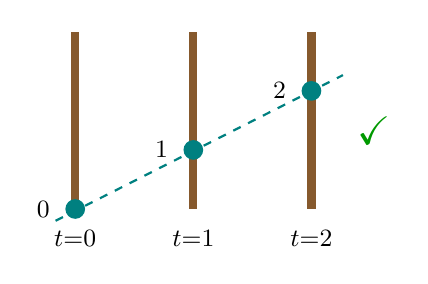
\begin{tikzpicture}[scale=0.5]
  % chopsticks at t=0, 1, 2 (visual: x=0, 3, 6)
  \draw[brown!70!black, line width=3pt] (0,0) -- (0,4.5);
  \draw[brown!70!black, line width=3pt] (3,0) -- (3,4.5);
  \draw[brown!70!black, line width=3pt] (6,0) -- (6,4.5);
  \node[below,font=\small] at (0,-0.3) {$t{=}0$};
  \node[below,font=\small] at (3,-0.3) {$t{=}1$};
  \node[below,font=\small] at (6,-0.3) {$t{=}2$};
  % marbles at heights = t values: 0, 1, 2 (scale by 1.5)
  \fill[teal] (0,0) circle (0.25);
  \fill[teal] (3,1.5) circle (0.25);
  \fill[teal] (6,3.0) circle (0.25);
  \node[left,font=\small] at (-0.4,0) {$0$};
  \node[left,font=\small] at (2.6,1.5) {$1$};
  \node[left,font=\small] at (5.6,3.0) {$2$};
  % diagonal line through marbles
  \draw[teal,thick,dashed] (-0.5,-0.3) -- (6.8,3.4);
  \node[green!60!black,font=\Large] at (7.6,2) {$\checkmark$};
\end{tikzpicture}
\end{center}

\vspace{0.3em}

The marbles trace out the line $h = t$. Perfect!

\vspace{0.3em}

In data space: the point $\tl{(0, 1, 2)}$ --- the chopstick positions themselves.

\end{frame}


% ADR: AUDIENCE EMOTION — now show BOTH special points plus the origin
% in data space. Three points determine a plane. This is the geometric
% reason why perfect data forms a plane — no algebra needed.
% The origin (0,0,0) corresponds to h(t) = 0 (no candle, trivially perfect).
\begin{frame}[fragile]{Three Points Determine the Plane}

\begin{columns}
\column{0.5\textwidth}
We found three perfect-data points:

\vspace{0.5em}

\begin{itemize}
\item $\mathbf{0} = (0,0,0)$

\small no candle $\to$ trivially perfect

\vspace{0.3em}

\item $\bl{(1, 1, 1)}$

\small level marbles $\to$ horizontal line

\vspace{0.3em}

\item $\tl{(0, 1, 2)}$

\small diagonal marbles $\to$ slope-1 line
\end{itemize}

\column{0.5\textwidth}
\begin{center}
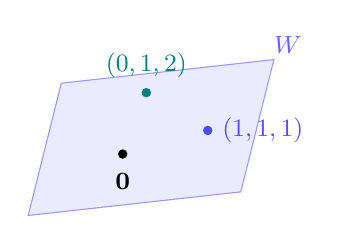
\begin{tikzpicture}[scale=0.6]
  % plane
  \fill[blue!8] (-1,-0.8) -- (3.5,-0.3) -- (4.2,2.5) -- (-0.3,2.0) -- cycle;
  \draw[blue!40] (-1,-0.8) -- (3.5,-0.3) -- (4.2,2.5) -- (-0.3,2.0) -- cycle;
  % origin
  \fill[black] (1.0,0.5) circle (0.1);
  \node[below,font=\small] at (1.0,0.3) {$\mathbf{0}$};
  % (1,1,1)
  \fill[blue!70] (2.8,1.0) circle (0.1);
  \node[right,font=\small,blue!70] at (2.9,1.0) {$(1,1,1)$};
  % (0,1,2)
  \fill[teal] (1.5,1.8) circle (0.1);
  \node[above,font=\small,teal] at (1.5,1.9) {$(0,1,2)$};
  % label
  \node[blue!60,font=\small] at (4.5,2.8) {$W$};
\end{tikzpicture}
\end{center}
\end{columns}

\vspace{0.5em}

Three points that don't lie on a line determine a \x{plane}.

This plane $W$ contains \x{all} perfect data.

\end{frame}


% ADR: AUDIENCE EMOTION — now explain WHY every perfect data is on this plane.
% Any line h = a + bt is a "mix" of the horizontal (constant a) and
% the diagonal (slope b). The marble heights are a*(1,1,1) + b*(0,1,2).
% Show this as: take the level marbles, scale by a, then add the diagonal
% marbles scaled by b. This is VISUAL mixing, not algebra.
\begin{frame}[fragile]{Every Perfect Line = A Mix of These Two}

\begin{center}
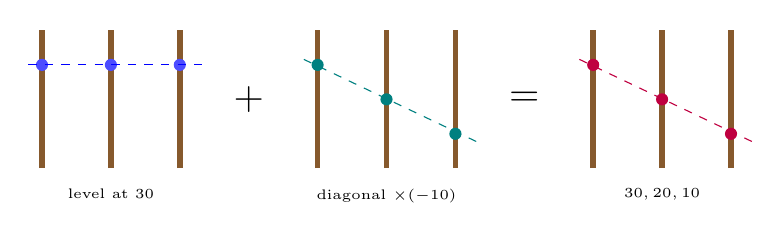
\begin{tikzpicture}[scale=0.35]
  % Level marbles (scaled by a=30)
  \draw[brown!70!black, line width=2pt] (0,0) -- (0,5);
  \draw[brown!70!black, line width=2pt] (2.5,0) -- (2.5,5);
  \draw[brown!70!black, line width=2pt] (5,0) -- (5,5);
  \fill[blue!70] (0,3.75) circle (0.22);
  \fill[blue!70] (2.5,3.75) circle (0.22);
  \fill[blue!70] (5,3.75) circle (0.22);
  \draw[blue,dashed] (-0.5,3.75) -- (5.8,3.75);
  \node[below,font=\tiny] at (2.5,-0.4) {level at $30$};

  % Plus sign
  \node[font=\Large] at (7.5,2.5) {$+$};

  % Diagonal marbles (scaled by b=-10)
  \begin{scope}[xshift=10cm]
  \draw[brown!70!black, line width=2pt] (0,0) -- (0,5);
  \draw[brown!70!black, line width=2pt] (2.5,0) -- (2.5,5);
  \draw[brown!70!black, line width=2pt] (5,0) -- (5,5);
  \fill[teal] (0,3.75) circle (0.22);
  \fill[teal] (2.5,2.5) circle (0.22);
  \fill[teal] (5,1.25) circle (0.22);
  \draw[teal,dashed] (-0.5,3.95) -- (5.8,0.95);
  \node[below,font=\tiny] at (2.5,-0.4) {diagonal $\times(-10)$};
  \end{scope}

  % Equals sign
  \node[font=\Large] at (17.5,2.5) {$=$};

  % Result: 30, 20, 10
  \begin{scope}[xshift=20cm]
  \draw[brown!70!black, line width=2pt] (0,0) -- (0,5);
  \draw[brown!70!black, line width=2pt] (2.5,0) -- (2.5,5);
  \draw[brown!70!black, line width=2pt] (5,0) -- (5,5);
  \fill[purple] (0,3.75) circle (0.22);
  \fill[purple] (2.5,2.5) circle (0.22);
  \fill[purple] (5,1.25) circle (0.22);
  \draw[purple,dashed] (-0.5,3.95) -- (5.8,0.95);
  \node[below,font=\tiny] at (2.5,-0.4) {$30, 20, 10$};
  \end{scope}
\end{tikzpicture}
\end{center}

\vspace{0.5em}

Any perfect line is a \x{mix} of ``level'' and ``diagonal.''

\vspace{0.3em}

All mixes of two directions $\to$ a \x{plane} in data space.

\end{frame}


% ADR: AUDIENCE EMOTION — the KEY correspondence picture.
% Left: scatter plot with many lines (messy). Right: data space with
% points on a plane (clean). Each line in the scatter plot becomes
% one point on the plane. The data point b is OFF the plane.
% This picture ties together both spaces and sets up the projection.
\begin{frame}[fragile]{Lines in Scatter Plot = Points on a Plane}

\begin{columns}
\column{0.45\textwidth}
\begin{center}
\textbf{Scatter plot}

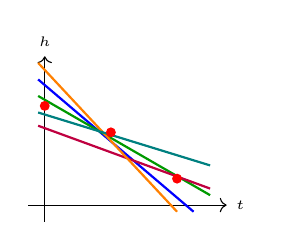
\begin{tikzpicture}[scale=0.42]
  \draw[->] (-0.5,0) -- (5.5,0) node[right] {\tiny $t$};
  \draw[->] (0,-0.5) -- (0,4.5) node[above] {\tiny $h$};
  \draw[blue,thick] (-0.2,3.8) -- (4.5,-0.2);
  \draw[green!60!black,thick] (-0.2,3.3) -- (5,0.3);
  \draw[purple,thick] (-0.2,2.4) -- (5,0.5);
  \draw[orange,thick] (-0.2,4.3) -- (4,-0.2);
  \draw[teal,thick] (-0.2,2.8) -- (5,1.2);
  \fill[red] (0,3) circle (0.15);
  \fill[red] (2,2.2) circle (0.15);
  \fill[red] (4,0.8) circle (0.15);
\end{tikzpicture}

\small Many lines, each a\\different ``perfect candle''
\end{center}

\column{0.1\textwidth}
\begin{center}
\vspace{2em}
\Large $\longleftrightarrow$
\end{center}

\column{0.45\textwidth}
\begin{center}
\textbf{Data space $\mathbb{R}^3$}

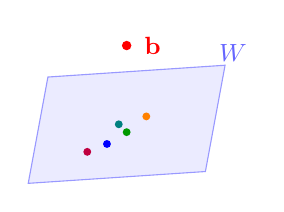
\begin{tikzpicture}[scale=0.5]
  \fill[blue!8] (-0.5,-0.5) -- (4,-0.2) -- (4.5,2.5) -- (0,2.2) -- cycle;
  \draw[blue!40] (-0.5,-0.5) -- (4,-0.2) -- (4.5,2.5) -- (0,2.2) -- cycle;
  \fill[blue] (1.5,0.5) circle (0.1);
  \fill[green!60!black] (2.0,0.8) circle (0.1);
  \fill[purple] (1.0,0.3) circle (0.1);
  \fill[orange] (2.5,1.2) circle (0.1);
  \fill[teal] (1.8,1.0) circle (0.1);
  \node[blue!60,font=\small] at (4.7,2.8) {$W$};
  \fill[red] (2.0,3.0) circle (0.12);
  \node[red,font=\small,right] at (2.2,3.0) {$\mathbf{b}$};
\end{tikzpicture}

\small Each line becomes\\one point on the plane $W$
\end{center}
\end{columns}

\vspace{0.5em}

Each line in the scatter plot is one point on the plane. Our data $\mathbf{b}$ is \x{off the plane}.

\end{frame}


% ADR: AUDIENCE EMOTION — name the plane Col(A). Minimal. Just the matrix
% with labeled columns tying back to the chopstick visuals.
\begin{frame}{Our Plane}

$$W = \operatorname{Col}\begin{pmatrix} 1 & 0 \\ 1 & 1 \\ 1 & 2 \end{pmatrix}$$

\vspace{0.3em}

\begin{center}
\renewcommand{\arraystretch}{1.2}
\begin{tabular}{cl}
Column 1: $(1, 1, 1)^T$ & $\leftarrow$ level marbles \\
Column 2: $(0, 1, 2)^T$ & $\leftarrow$ chopstick positions
\end{tabular}
\end{center}

\vspace{0.5em}

\x{Move the chopsticks $\to$ change column 2 $\to$ change the plane.}

\end{frame}


% ADR: AUDIENCE EMOTION — the geometric picture. Show the plane with
% the data point NOT on it. This is the setup for the projection insight.
\begin{frame}[fragile]{The Picture}

\begin{center}
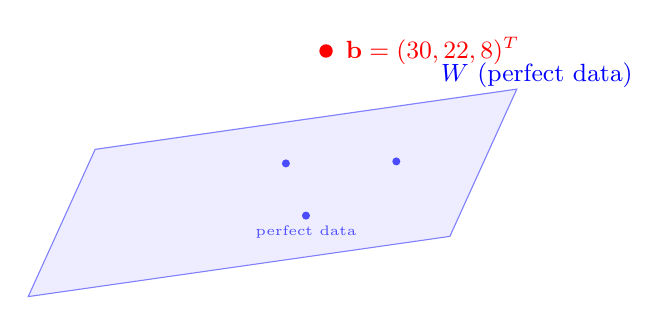
\begin{tikzpicture}[scale=0.85]
  % Draw a plane (parallelogram)
  \coordinate (O) at (0,0);
  \coordinate (V1) at (3.5,0.5);
  \coordinate (V2) at (1.0,2.2);

  \coordinate (A) at ($(O) - 0.6*(V1) - 0.4*(V2)$);
  \coordinate (B) at ($(O) + 1.2*(V1) - 0.4*(V2)$);
  \coordinate (C) at ($(O) + 1.2*(V1) + 0.6*(V2)$);
  \coordinate (D) at ($(O) - 0.6*(V1) + 0.6*(V2)$);

  \fill[blue!10, opacity=0.7] (A) -- (B) -- (C) -- (D) -- cycle;
  \draw[blue!50] (A) -- (B) -- (C) -- (D) -- cycle;

  \node[blue, font=\small] at ($(C) + (0.3,0.2)$) {$W$ (perfect data)};

  % points on the plane
  \fill[blue!70] ($(O) + 0.5*(V1) - 0.1*(V2)$) circle (0.06);
  \fill[blue!70] ($(O) + 0.3*(V1) + 0.3*(V2)$) circle (0.06);
  \fill[blue!70] ($(O) + 0.8*(V1) + 0.2*(V2)$) circle (0.06);

  % the data point, OFF the plane
  \coordinate (b) at ($(O) + 0.5*(V1) + 0.2*(V2) + (0,1.8)$);
  \fill[red] (b) circle (0.1);
  \node[red, right, font=\small] at ($(b) + (0.15,0)$) {$\mathbf{b} = (30, 22, 8)^T$};

  \node[blue!70, font=\tiny, below] at ($(O) + 0.5*(V1) - 0.1*(V2)$) {perfect data};
\end{tikzpicture}
\end{center}

\vspace{0.3em}

Our data $\mathbf{b}$ is \x{not on the plane} $W$ (the candle didn't burn perfectly).

\end{frame}


% ADR: AUDIENCE EMOTION — summary of Step B.
\begin{frame}{Model = A Plane}

\begin{center}
\large
All perfect lines in the scatter plot

$\Big\Downarrow$

\vspace{0.5em}

A plane $W$ in data space $\mathbb{R}^3$
\end{center}

\vspace{0.5em}

Which plane? That depends on \x{where you put the chopsticks} (the measurement times).

\vspace{0.3em}

Our chopsticks at $t = 0, 1, 2$ give: $W = \operatorname{Col}\begin{pmatrix} 1 & 0 \\ 1 & 1 \\ 1 & 2 \end{pmatrix}$

\end{frame}


% ADR: AUDIENCE EMOTION — the translation table. Pull Steps A and B together.
% Bridge to Step C. The "???" creates tension for the next section.
\begin{frame}{The Translation So Far}

\renewcommand{\arraystretch}{1.4}
\begin{center}
\begin{tabular}{c|c}
\textbf{Candle Problem} & \textbf{Geometry in $\mathbb{R}^3$} \\
\hline
Measurements $(30, 22, 8)$ & A point $\mathbf{b} \in \mathbb{R}^3$ \\
Model $h(t) = a+bt$ & A plane $W \subseteq \mathbb{R}^3$ \\
Data has errors & $\mathbf{b}$ is not on $W$ \\
\hline
Find the best line & \x{???}
\end{tabular}
\end{center}

\vspace{1em}

What does ``find the best line'' become in geometry?

\end{frame}


% ═══════════════════════════════════════
% §3 ERROR = DISTANCE
% ADR: DESIGN DECISION — this section connects the two spaces:
%   scatter-plot error (sum of squared gaps) = data-space distance².
% Students cannot SEE this connection in pictures alone — the scatter
% plot is 2D, the data space is 3D. So we show BOTH pictures side by
% side, state the equality, and let the Pythagorean theorem do the work.
% Once error = distance², minimizing error = finding the closest point
% on the plane = dropping a perpendicular = ORTHOGONAL PROJECTION.
% This is the "aha" moment of the entire lecture.
% Structure: show both quantities visually → state equality →
%   minimize error = minimize distance → closest point = perpendicular
%   → "we already know how to do this!" → callback to Lecture 10.
% ═══════════════════════════════════════
\section{Error = Distance}


% ADR: AUDIENCE EMOTION — show the scatter plot error visually.
% Pick a specific line, draw the gaps, write the sum of squares as
% pure arithmetic. No a, no b. Just numbers.
\begin{frame}[fragile]{Error in the Scatter Plot}

Pick a line. Measure the three gaps:

\vspace{0.3em}

\begin{center}
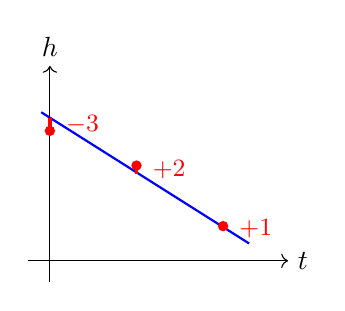
\begin{tikzpicture}[scale=0.55]
  \draw[->] (-0.5,0) -- (5.5,0) node[right] {$t$};
  \draw[->] (0,-0.5) -- (0,4.5) node[above] {$h$};
  % a candidate line (not the best): h=33-13t
  % t=0→x=0: y=3.3, t=1→x=2: y=2.0, t=2→x=4: y=0.7
  \draw[blue,thick] (-0.2,3.43) -- (4.6,0.4);
  % gaps: data(30,22,8) - line(33,20,7) = (-3,+2,+1)
  \draw[red,very thick] (0,3.3) -- (0,3.0);
  \draw[red,very thick] (2,2.0) -- (2,2.2);
  \draw[red,very thick] (4,0.7) -- (4,0.8);
  \node[red,font=\small,right] at (0.15,3.15) {$-3$};
  \node[red,font=\small,right] at (2.15,2.1) {$+2$};
  \node[red,font=\small,right] at (4.15,0.75) {$+1$};
  % data points
  \fill[red] (0,3) circle (0.12);
  \fill[red] (2,2.2) circle (0.12);
  \fill[red] (4,0.8) circle (0.12);
\end{tikzpicture}
\end{center}

\vspace{0.3em}

$$\text{Error} = (-3)^2 + (+2)^2 + (+1)^2 = 9 + 4 + 1 = 14$$

\end{frame}


% ADR: AUDIENCE EMOTION — now show the SAME situation in data space.
% The data point b is off the plane. The chosen line corresponds to
% a point on the plane. The distance between them is related to the error.
% Draw b, the plane, and a line from b to the chosen point on W.
\begin{frame}[fragile]{Distance in Data Space}

That same line is a point on the plane $W$. How far is it from $\mathbf{b}$?

\vspace{0.3em}

\begin{center}
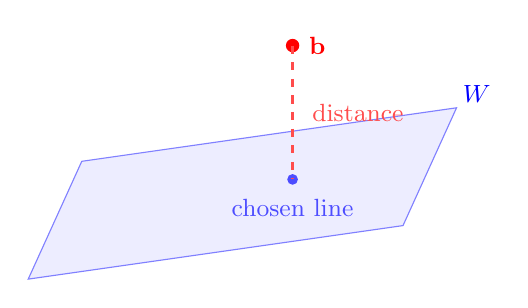
\begin{tikzpicture}[scale=0.85]
  % plane
  \coordinate (O) at (0,0);
  \coordinate (V1) at (3.5,0.5);
  \coordinate (V2) at (1.0,2.2);
  \coordinate (A) at ($(O) - 0.5*(V1) - 0.3*(V2)$);
  \coordinate (B) at ($(O) + 1.1*(V1) - 0.3*(V2)$);
  \coordinate (C) at ($(O) + 1.1*(V1) + 0.5*(V2)$);
  \coordinate (D) at ($(O) - 0.5*(V1) + 0.5*(V2)$);
  \fill[blue!10, opacity=0.7] (A) -- (B) -- (C) -- (D) -- cycle;
  \draw[blue!50] (A) -- (B) -- (C) -- (D) -- cycle;
  \node[blue,font=\small] at ($(C) + (0.3,0.2)$) {$W$};

  % a point on the plane (the chosen line)
  \coordinate (p) at ($(O) + 0.5*(V1) + 0.15*(V2)$);
  \fill[blue!70] (p) circle (0.08);
  \node[blue!70,font=\small,below] at ($(p) + (0,-0.15)$) {chosen line};

  % data point
  \coordinate (b) at ($(O) + 0.5*(V1) + 0.15*(V2) + (0,2.0)$);
  \fill[red] (b) circle (0.1);
  \node[red,font=\small,right] at ($(b) + (0.1,0)$) {$\mathbf{b}$};

  % distance line
  \draw[red!70,thick,dashed] (b) -- (p);
  \node[red!70,font=\small,right] at ($(b)!0.5!(p) + (0.15,0)$) {distance};
\end{tikzpicture}
\end{center}

\vspace{0.3em}

$$\text{Distance}^2 = (30-33)^2 + (22-20)^2 + (8-7)^2 = 9 + 4 + 1 = \x{14}$$

\end{frame}


% ADR: AUDIENCE EMOTION — the punchline: they're the SAME number!
% Show both pictures side by side, with "= 6" under each.
% This is the key connection between the two spaces.
\begin{frame}[fragile]{They Are the Same!}

\begin{columns}
\column{0.45\textwidth}
\begin{center}
\textbf{Scatter plot}

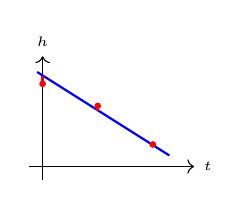
\begin{tikzpicture}[scale=0.35]
  \draw[->] (-0.5,0) -- (5.5,0) node[right] {\tiny $t$};
  \draw[->] (0,-0.5) -- (0,4) node[above] {\tiny $h$};
  \draw[blue,thick] (-0.2,3.43) -- (4.6,0.4);
  \draw[red,very thick] (0,3.3) -- (0,3.0);
  \draw[red,very thick] (2,2.0) -- (2,2.2);
  \draw[red,very thick] (4,0.7) -- (4,0.8);
  \fill[red] (0,3) circle (0.12);
  \fill[red] (2,2.2) circle (0.12);
  \fill[red] (4,0.8) circle (0.12);
\end{tikzpicture}

\small gap$_1^2$ + gap$_2^2$ + gap$_3^2$

$= 9 + 4 + 1 = \mathbf{14}$
\end{center}

\column{0.1\textwidth}
\begin{center}
\vspace{1.5em}
\Large $=$
\end{center}

\column{0.45\textwidth}
\begin{center}
\textbf{Data space}

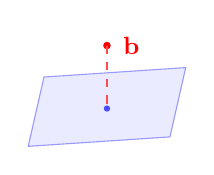
\begin{tikzpicture}[scale=0.4]
  \fill[blue!8] (-1,-0.5) -- (3.5,-0.2) -- (4,2) -- (-0.5,1.7) -- cycle;
  \draw[blue!40] (-1,-0.5) -- (3.5,-0.2) -- (4,2) -- (-0.5,1.7) -- cycle;
  \fill[blue!70] (1.5,0.7) circle (0.1);
  \fill[red] (1.5,2.7) circle (0.12);
  \draw[red!70,thick,dashed] (1.5,2.7) -- (1.5,0.7);
  \node[red,font=\small,right] at (1.7,2.7) {$\mathbf{b}$};
\end{tikzpicture}

\small distance$^2$

$= 9 + 4 + 1 = \mathbf{14}$
\end{center}
\end{columns}

\vspace{0.5em}

The sum of squared gaps in the scatter plot \x{equals} the squared distance in data space.

\vspace{0.3em}

\small (Each gap becomes one coordinate of the difference vector. Pythagorean theorem does the rest.)

\end{frame}


% ADR: AUDIENCE EMOTION — the consequence: minimize error = minimize distance.
% Draw the plane with b above it, and ask: which point on W is closest?
\begin{frame}[fragile]{Minimize Error = Minimize Distance}

Finding the \x{best line} means finding the point on $W$ \x{closest to $\mathbf{b}$}.

\vspace{0.5em}

\begin{center}
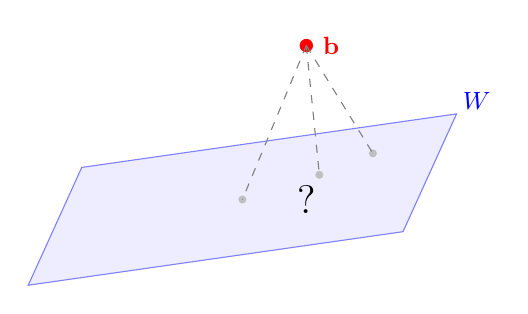
\begin{tikzpicture}[scale=0.85]
  % plane
  \coordinate (O) at (0,0);
  \coordinate (V1) at (3.5,0.5);
  \coordinate (V2) at (1.0,2.2);
  \coordinate (A) at ($(O) - 0.5*(V1) - 0.3*(V2)$);
  \coordinate (B) at ($(O) + 1.1*(V1) - 0.3*(V2)$);
  \coordinate (C) at ($(O) + 1.1*(V1) + 0.5*(V2)$);
  \coordinate (D) at ($(O) - 0.5*(V1) + 0.5*(V2)$);
  \fill[blue!10, opacity=0.7] (A) -- (B) -- (C) -- (D) -- cycle;
  \draw[blue!50] (A) -- (B) -- (C) -- (D) -- cycle;
  \node[blue,font=\small] at ($(C) + (0.3,0.2)$) {$W$};

  % several candidate points on the plane
  \coordinate (p1) at ($(O) + 0.3*(V1) + 0.1*(V2)$);
  \coordinate (p2) at ($(O) + 0.6*(V1) + 0.2*(V2)$);
  \coordinate (p3) at ($(O) + 0.8*(V1) + 0.3*(V2)$);
  \fill[gray!50] (p1) circle (0.06);
  \fill[gray!50] (p2) circle (0.06);
  \fill[gray!50] (p3) circle (0.06);

  % data point
  \coordinate (b) at ($(O) + 0.55*(V1) + 0.18*(V2) + (0,2.0)$);
  \fill[red] (b) circle (0.1);
  \node[red,font=\small,right] at ($(b) + (0.1,0)$) {$\mathbf{b}$};

  % dashed lines from b to candidates
  \draw[gray,dashed,thin] (b) -- (p1);
  \draw[gray,dashed,thin] (b) -- (p2);
  \draw[gray,dashed,thin] (b) -- (p3);

  % question mark at the closest point region
  \node[font=\Large] at ($(O) + 0.55*(V1) + 0.18*(V2) + (0,-0.3)$) {?};
\end{tikzpicture}
\end{center}

\vspace{0.3em}

Which point on the plane $W$ has the \x{shortest} distance to $\mathbf{b}$?

\end{frame}


% ADR: AUDIENCE EMOTION — the AHA moment. Drop a perpendicular!
% The closest point on a plane is the foot of the perpendicular.
% Draw b, the plane, a vertical line down to the foot, and a right angle mark.
\begin{frame}[fragile]{Drop a Perpendicular!}

\begin{center}
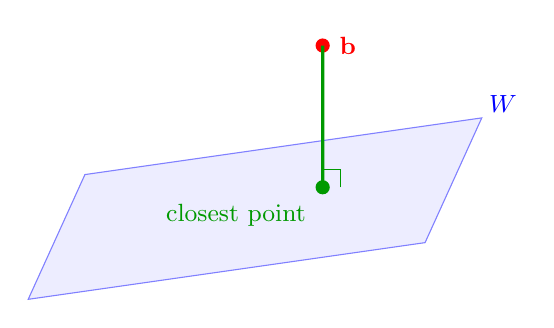
\begin{tikzpicture}[scale=0.9]
  % plane
  \coordinate (O) at (0,0);
  \coordinate (V1) at (3.5,0.5);
  \coordinate (V2) at (1.0,2.2);
  \coordinate (A) at ($(O) - 0.5*(V1) - 0.3*(V2)$);
  \coordinate (B) at ($(O) + 1.1*(V1) - 0.3*(V2)$);
  \coordinate (C) at ($(O) + 1.1*(V1) + 0.5*(V2)$);
  \coordinate (D) at ($(O) - 0.5*(V1) + 0.5*(V2)$);
  \fill[blue!10, opacity=0.7] (A) -- (B) -- (C) -- (D) -- cycle;
  \draw[blue!50] (A) -- (B) -- (C) -- (D) -- cycle;
  \node[blue,font=\small] at ($(C) + (0.3,0.2)$) {$W$};

  % foot of perpendicular
  \coordinate (foot) at ($(O) + 0.55*(V1) + 0.18*(V2)$);
  \fill[green!60!black] (foot) circle (0.1);
  \node[green!60!black,font=\small,below left] at ($(foot) + (-0.1,-0.1)$) {closest point};

  % data point
  \coordinate (b) at ($(foot) + (0,2.0)$);
  \fill[red] (b) circle (0.1);
  \node[red,font=\small,right] at ($(b) + (0.1,0)$) {$\mathbf{b}$};

  % perpendicular line
  \draw[green!60!black,very thick] (b) -- (foot);

  % right angle mark
  \draw[green!60!black] ($(foot) + (0.25,0)$) -- ($(foot) + (0.25,0.25)$) -- ($(foot) + (0,0.25)$);
\end{tikzpicture}
\end{center}

\vspace{0.5em}

The closest point on a plane is always the \x{foot of the perpendicular}.

\vspace{0.3em}

This is the \x{orthogonal projection} of $\mathbf{b}$ onto $W$.

\end{frame}


% ADR: AUDIENCE EMOTION — the callback to Lecture 10. This is the emotional
% payoff: "we already learned how to do this!" The projection formula
% from Lecture 10 solves the candle problem.
\begin{frame}{We Already Know How to Do This!}

\x{Callback} (Lecture 10): The orthogonal projection onto $\operatorname{Col}(B)$ is

$$P = B(B^TB)^{-1}B^T$$

\vspace{0.5em}

For our candle, $B = \begin{pmatrix} 1 & 0 \\ 1 & 1 \\ 1 & 2 \end{pmatrix}$.

\vspace{0.5em}

The best line is encoded in $P\mathbf{b}$ --- the projection of our data onto the perfect-data plane.

\vspace{1em}

\x{The candle problem is solved by a projection.}

\end{frame}


% ADR: AUDIENCE EMOTION — the complete translation table. Now the "???" is filled.
\begin{frame}{The Complete Translation}

\renewcommand{\arraystretch}{1.4}
\begin{center}
\begin{tabular}{c|c}
\textbf{Candle Problem} & \textbf{Geometry in $\mathbb{R}^3$} \\
\hline
Measurements $(30, 22, 8)$ & A point $\mathbf{b} \in \mathbb{R}^3$ \\
Model $h(t) = a+bt$ & A plane $W \subseteq \mathbb{R}^3$ \\
Data has errors & $\mathbf{b}$ is not on $W$ \\
Sum of squared gaps & Distance$^2$ from $\mathbf{b}$ to $W$ \\
\hline
Find the best line & \x{Orthogonal projection of $\mathbf{b}$ onto $W$}
\end{tabular}
\end{center}

\end{frame}


% ═══════════════════════════════════════
% §4 SOLVING THE CANDLE PROBLEM
% ADR: DESIGN DECISION — this section performs the full computation.
% Every step is shown with underbrace labels connecting abstract symbols
% to the candle problem. The key insight: P_W b = B x̂ where x̂ = (a,b)^T
% gives the regression coefficients DIRECTLY. We never need the 3×3
% projection matrix P — only the 2×2 system (B^T B) x̂ = B^T b.
% Structure: set up formula → identify B and b → compute B^T B →
%   compute B^T b → solve 2×2 system → read off a, b → draw the line.
% Cross-filling is shown for (B^T B)^{-1} to connect with Lecture 10.
% ═══════════════════════════════════════
\section{Solving the Candle Problem}


% ADR: AUDIENCE EMOTION — recall the formula with explicit underbrace labels.
% Every symbol must be tied to the candle problem. No orphan notation.
\begin{frame}{The Formula}

\x{Callback} (Lecture 10): The orthogonal projection onto $\operatorname{Col}(B)$ is

$$P_W = B(B^TB)^{-1}B^T$$

\vspace{0.3em}

The best data (closest point on $W$ to $\mathbf{b}$) is:

$$P_W\mathbf{b} = \underbrace{B}_{\text{columns of }W} \underbrace{(B^TB)^{-1}B^T\mathbf{b}}_{\text{coefficients}}$$

\vspace{0.5em}

Write $\hat{\mathbf{x}} = (B^TB)^{-1}B^T\mathbf{b}$. Then $P_W\mathbf{b} = B\hat{\mathbf{x}}$.

\vspace{0.3em}

\x{$\hat{\mathbf{x}}$ tells us the regression coefficients directly!}

\end{frame}


% ADR: AUDIENCE EMOTION — write down B and b explicitly, with every entry labeled.
\begin{frame}{Our Ingredients}

$$\underbrace{B}_{\text{perfect data matrix}} = \begin{pmatrix} 1 & 0 \\ 1 & 1 \\ 1 & 2 \end{pmatrix} \qquad \underbrace{\mathbf{b}}_{\text{observed data}} = \begin{pmatrix} 30 \\ 22 \\ 8 \end{pmatrix}$$

\vspace{0.5em}

\begin{center}
\renewcommand{\arraystretch}{1.3}
\begin{tabular}{c|cc|c}
& \small col 1 & \small col 2 & \small data \\
\hline
$t = 0$ & $1$ & $0$ & $30$ \\
$t = 1$ & $1$ & $1$ & $22$ \\
$t = 2$ & $1$ & $2$ & $8$
\end{tabular}
\end{center}

\vspace{0.3em}

Column 1 = level marbles $(1,1,1)^T$. \quad Column 2 = chopstick positions $(0,1,2)^T$.

\end{frame}


% ADR: AUDIENCE EMOTION — the key observation: x̂ = (a, slope)^T.
% Show that B x̂ is literally the perfect data for line h = a + slope*t.
\begin{frame}{What Does $\hat{\mathbf{x}}$ Mean?}

Write $\hat{\mathbf{x}} = \begin{pmatrix} a \\ b \end{pmatrix}$. Then:

$$B\hat{\mathbf{x}} = \begin{pmatrix} 1 & 0 \\ 1 & 1 \\ 1 & 2 \end{pmatrix}\begin{pmatrix} a \\ b \end{pmatrix} = \begin{pmatrix} a \\ a + b \\ a + 2b \end{pmatrix} = \begin{pmatrix} h(0) \\ h(1) \\ h(2) \end{pmatrix}$$

\vspace{0.5em}

for the line $h(t) = a + bt$.

\vspace{0.5em}

\x{Finding $\hat{\mathbf{x}}$ gives us the intercept $a$ and the slope $b$ directly.}

\vspace{0.3em}

We don't need the $3 \times 3$ projection matrix $P_W$ at all!

\end{frame}


% ADR: AUDIENCE EMOTION — set up the computation x̂ = (B^T B)^{-1} B^T b.
% Key: we compute (B^T B)^{-1} × (B^T b) by simultaneous row operations.
% Format: equality chain, NOT augmented matrix. Follows Lecture 1–2 convention.
\begin{frame}{How to Compute $\hat{\mathbf{x}}$}

We need:

$$\hat{\mathbf{x}} = \underbrace{(B^TB)^{-1}}_{\text{invertible!}}\underbrace{B^T\mathbf{b}}_{\text{a vector}}$$

\vspace{0.5em}

\x{Callback} (Lectures 1--2): Apply \x{simultaneous row operations} to both matrices until the left one becomes $I$. The right side becomes $(B^TB)^{-1}B^T\mathbf{b}$.

\end{frame}


% ADR: AUDIENCE EMOTION — compute B^T B step by step.
% Show the multiplication with every entry labeled.
\begin{frame}{Step 1: Compute $B^TB$}

$$B^TB = \underbrace{\begin{pmatrix} 1 & 1 & 1 \\ 0 & 1 & 2 \end{pmatrix}}_{B^T}\underbrace{\begin{pmatrix} 1 & 0 \\ 1 & 1 \\ 1 & 2 \end{pmatrix}}_{B}$$

\vspace{0.5em}

$$= \begin{pmatrix} 1+1+1 & 0+1+2 \\ 0+1+2 & 0+1+4 \end{pmatrix} = \begin{pmatrix} 3 & 3 \\ 3 & 5 \end{pmatrix}$$

\vspace{0.5em}

A $2 \times 2$ symmetric matrix. \; ($B$ has full column rank, so $B^TB$ is \x{invertible}.)

\end{frame}


% ADR: AUDIENCE EMOTION — compute B^T b step by step.
\begin{frame}{Step 2: Compute $B^T\mathbf{b}$}

$$B^T\mathbf{b} = \begin{pmatrix} 1 & 1 & 1 \\ 0 & 1 & 2 \end{pmatrix}\begin{pmatrix} 30 \\ 22 \\ 8 \end{pmatrix}$$

\vspace{0.5em}

$$= \begin{pmatrix} 30 + 22 + 8 \\ 0 + 22 + 16 \end{pmatrix} = \begin{pmatrix} 60 \\ 38 \end{pmatrix}$$

\vspace{0.5em}

Entry 1: sum of all measurements. \quad Entry 2: weighted sum (by chopstick positions).

\end{frame}


% ADR: AUDIENCE EMOTION — simultaneous row operations, equality format.
% Every line is a strict equality. No augmented matrices.
% Follows the convention from Lectures 1–2 (rowoperation.tex).
\begin{frame}{Step 3: Simultaneous Row Operations}

\textbf{Setup:}
$$\hat{\mathbf{x}} = \begin{pmatrix} 3 & 3 \\ 3 & 5 \end{pmatrix}^{-1}\begin{pmatrix} 60 \\ 38 \end{pmatrix}$$

\vspace{0.3em}

\textbf{Step 1:} $r_2 \to r_2 - r_1$
$$= \begin{pmatrix} 3 & 3 \\ 0 & 2 \end{pmatrix}^{-1}\begin{pmatrix} 60 \\ -22 \end{pmatrix}$$

\textbf{Step 2:} $r_2 \to \frac{1}{2}r_2$
$$= \begin{pmatrix} 3 & 3 \\ 0 & 1 \end{pmatrix}^{-1}\begin{pmatrix} 60 \\ -11 \end{pmatrix}$$

\end{frame}


% ADR: AUDIENCE EMOTION — finish row reduction. Every step is an equality.
\begin{frame}{Step 3: Simultaneous Row Operations (continued)}

\textbf{Step 3:} $r_1 \to r_1 - 3r_2$
$$\hat{\mathbf{x}} = \begin{pmatrix} 3 & 0 \\ 0 & 1 \end{pmatrix}^{-1}\begin{pmatrix} 93 \\ -11 \end{pmatrix}$$

\textbf{Step 4:} $r_1 \to \frac{1}{3}r_1$
$$= \begin{pmatrix} 1 & 0 \\ 0 & 1 \end{pmatrix}^{-1}\begin{pmatrix} 31 \\ -11 \end{pmatrix} = \begin{pmatrix} \x{31} \\ \x{-11} \end{pmatrix}$$

\vspace{0.5em}

$$\hat{\mathbf{x}} = \begin{pmatrix} a \\ b \end{pmatrix} = \begin{pmatrix} 31 \\ -11 \end{pmatrix}$$

\end{frame}


% ADR: AUDIENCE EMOTION — the answer! State it big, with the line equation
% and the meaning of each coefficient.
\begin{frame}{The Best Line}

$$\hat{\mathbf{x}} = \begin{pmatrix} a \\ b \end{pmatrix} = \begin{pmatrix} 31 \\ -11 \end{pmatrix}$$

\vspace{0.5em}

The best-fitting line is:

$$\boxed{h(t) = 31 - 11t}$$

\vspace{0.5em}

\begin{center}
\renewcommand{\arraystretch}{1.3}
\begin{tabular}{cl}
$a = 31$ & $\leftarrow$ predicted height at $t = 0$ \\
$b = -11$ & $\leftarrow$ the candle loses $11$ cm per hour
\end{tabular}
\end{center}

\end{frame}


% ADR: AUDIENCE EMOTION — check: compute the predicted values and errors.
% Students see the regression line is NOT perfect — it doesn't pass through
% any data point. But it's the CLOSEST.
\begin{frame}{Check: Predicted vs.\ Actual}

\renewcommand{\arraystretch}{1.4}
\begin{center}
\begin{tabular}{c|c|c|c}
$t$ & Actual $h$ & Predicted $31 - 11t$ & Error \\
\hline
$0$ & $30$ & $31$ & $-1$ \\
$1$ & $22$ & $20$ & $+2$ \\
$2$ & $8$ & $9$ & $-1$
\end{tabular}
\end{center}

\vspace{0.5em}

$$\text{Sum of squared errors} = (-1)^2 + 2^2 + (-1)^2 = 1 + 4 + 1 = \x{6}$$

\vspace{0.3em}

No line can do better than error $= 6$. This is the \x{minimum}.

\end{frame}


% ADR: AUDIENCE EMOTION — draw the line on the scatter plot. Visual payoff.
\begin{frame}[fragile]{The Best Line on the Scatter Plot}

\begin{center}
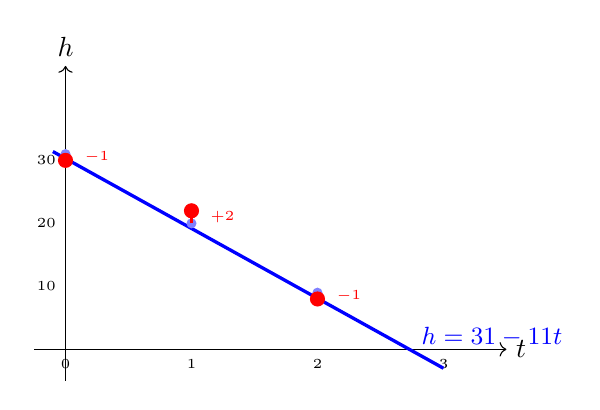
\begin{tikzpicture}[scale=0.8]
  % axes (t-scale: 1 unit = 2 on x-axis)
  \draw[->] (-0.5,0) -- (7,0) node[right] {$t$};
  \draw[->] (0,-0.5) -- (0,4.5) node[above] {$h$};
  \foreach \x in {0,1,2,3} \node[below,font=\tiny] at (2*\x,0) {\x};
  \node[left,font=\tiny] at (0,1) {10};
  \node[left,font=\tiny] at (0,2) {20};
  \node[left,font=\tiny] at (0,3) {30};
  % best line: h=31-11t. At t=0: 31→y=3.1, t=3: -2→y=-0.2
  \draw[blue,very thick] (-0.2,3.14) -- (6,-0.3);
  \node[blue,font=\small,right] at (5.5,0.2) {$h = 31 - 11t$};
  % predicted points (on the line)
  \fill[blue!50] (0,3.1) circle (0.08);
  \fill[blue!50] (2,2.0) circle (0.08);
  \fill[blue!50] (4,0.9) circle (0.08);
  % error bars
  \draw[red,thick,dashed] (0,3.1) -- (0,3.0);
  \draw[red,thick,dashed] (2,2.0) -- (2,2.2);
  \draw[red,thick,dashed] (4,0.9) -- (4,0.8);
  \node[red,font=\tiny,right] at (0.15,3.05) {$-1$};
  \node[red,font=\tiny,right] at (2.15,2.1) {$+2$};
  \node[red,font=\tiny,right] at (4.15,0.85) {$-1$};
  % data points (on top)
  \fill[red] (0,3) circle (0.12);
  \fill[red] (2,2.2) circle (0.12);
  \fill[red] (4,0.8) circle (0.12);
\end{tikzpicture}
\end{center}

\vspace{0.3em}

The line doesn't pass through any data point --- but it's the \x{closest} any line can get.

\end{frame}


% ADR: AUDIENCE EMOTION — now show the cross-filling approach. This connects
% to Lecture 10's technique and shows how to decompose the projection.
\begin{frame}{Bonus: Find $(B^TB)^{-1}$}

$$(B^TB)^{-1} = \begin{pmatrix} 3 & 3 \\ 3 & 5 \end{pmatrix}^{-1}\begin{pmatrix} 1 & 0 \\ 0 & 1 \end{pmatrix}$$

$r_2 \to r_2 - r_1$, \; $r_2 \to \frac{1}{2}r_2$, \; $r_1 \to r_1 - 3r_2$, \; $r_1 \to \frac{1}{3}r_1$:

$$= \begin{pmatrix} 1 & 0 \\ 0 & 1 \end{pmatrix}^{-1}\begin{pmatrix} \frac{5}{6} & -\frac{1}{2} \\[3pt] -\frac{1}{2} & \frac{1}{2} \end{pmatrix} = \frac{1}{6}\begin{pmatrix} \pvt{5} & \crs{-3} \\ \crs{-3} & 3 \end{pmatrix}$$

\end{frame}


% ADR: AUDIENCE EMOTION — cross-fill the inverse to get orthogonal basis.
\begin{frame}{Bonus: Cross-Fill $(B^TB)^{-1}$}

\x{Callback} (Lecture 10, \S4): Diagonally cross-fill $(B^TB)^{-1}$:

\vspace{0.3em}

Pivot $(\pvt{1},\pvt{1})$, value $= \pvt{\frac{5}{6}}$. Read off column 1: $\mathbf{d}_1 \propto \begin{pmatrix} 5 \\ -3 \end{pmatrix}$

$$B\mathbf{d}_1 = \begin{pmatrix} 1 & 0 \\ 1 & 1 \\ 1 & 2 \end{pmatrix}\begin{pmatrix} 5 \\ -3 \end{pmatrix} = \bl{\begin{pmatrix} 5 \\ 2 \\ -1 \end{pmatrix}}$$

\vspace{0.3em}

Remainder pivot at $(2,2)$: $\mathbf{d}_2 \propto \begin{pmatrix} 0 \\ 1 \end{pmatrix}$

$$B\mathbf{d}_2 = \begin{pmatrix} 1 & 0 \\ 1 & 1 \\ 1 & 2 \end{pmatrix}\begin{pmatrix} 0 \\ 1 \end{pmatrix} = \rd{\begin{pmatrix} 0 \\ 1 \\ 2 \end{pmatrix}}$$

\end{frame}


% ADR: AUDIENCE EMOTION — verify orthogonality and connect to the projection.
\begin{frame}{Orthogonal Basis for the Perfect-Data Plane}

$$\bl{\begin{pmatrix} 5 \\ 2 \\ -1 \end{pmatrix}}^T \rd{\begin{pmatrix} 0 \\ 1 \\ 2 \end{pmatrix}} = 0 + 2 - 2 = 0 \quad \checkmark$$

\vspace{0.5em}

$\left\{\bl{\begin{pmatrix} 5 \\ 2 \\ -1 \end{pmatrix}}, \rd{\begin{pmatrix} 0 \\ 1 \\ 2 \end{pmatrix}}\right\}$ is an \x{orthogonal basis} for the perfect-data plane $W$.

\vspace{0.5em}

\small (Same as Lecture 10, \S4 example --- same matrix $B$!)

\end{frame}


% ADR: AUDIENCE EMOTION — final answer with prediction.
\begin{frame}[fragile]{Prediction: When Does the Candle Burn Out?}

Our best line: $h(t) = 31 - 11t$.

\vspace{0.5em}

\begin{center}
\begin{tikzpicture}[scale=0.8]
  \draw[->] (-0.5,0) -- (7,0) node[right] {$t$};
  \draw[->] (0,-0.5) -- (0,4.5) node[above] {$h$};
  \foreach \x in {0,1,2,3} \node[below,font=\tiny] at (2*\x,0) {\x};
  \node[left,font=\tiny] at (0,1) {10};
  \node[left,font=\tiny] at (0,2) {20};
  \node[left,font=\tiny] at (0,3) {30};
  % best line extended
  \draw[blue,thick] (-0.2,3.14) -- (5.8,-0.1);
  % data points
  \fill[red] (0,3) circle (0.1);
  \fill[red] (2,2.2) circle (0.1);
  \fill[red] (4,0.8) circle (0.1);
  % burn-out point: h=0 → t=31/11 ≈ 2.82 → x=5.64
  \fill[green!60!black] (5.64,0) circle (0.12);
  \node[green!60!black,font=\small,above] at (5.64,0.15) {$t = \frac{31}{11} \approx 2.8$};
  \draw[green!60!black,dashed] (5.64,0) -- (5.64,-0.3);
\end{tikzpicture}
\end{center}

\vspace{0.3em}

Set $h(t) = 0$: \quad $31 - 11t = 0$ \quad $\Longrightarrow$ \quad $t = \frac{31}{11} \approx 2.8$ hours.

\vspace{0.3em}

\x{The candle burns out in about $2$ hours $48$ minutes.}

\end{frame}


\end{document}
